% Options for packages loaded elsewhere
\PassOptionsToPackage{unicode}{hyperref}
\PassOptionsToPackage{hyphens}{url}
\PassOptionsToPackage{dvipsnames,svgnames,x11names}{xcolor}
%
\documentclass[
  letterpaper,
  DIV=11,
  numbers=noendperiod]{scrartcl}

\usepackage{amsmath,amssymb}
\usepackage{lmodern}
\usepackage{iftex}
\ifPDFTeX
  \usepackage[T1]{fontenc}
  \usepackage[utf8]{inputenc}
  \usepackage{textcomp} % provide euro and other symbols
\else % if luatex or xetex
  \usepackage{unicode-math}
  \defaultfontfeatures{Scale=MatchLowercase}
  \defaultfontfeatures[\rmfamily]{Ligatures=TeX,Scale=1}
\fi
% Use upquote if available, for straight quotes in verbatim environments
\IfFileExists{upquote.sty}{\usepackage{upquote}}{}
\IfFileExists{microtype.sty}{% use microtype if available
  \usepackage[]{microtype}
  \UseMicrotypeSet[protrusion]{basicmath} % disable protrusion for tt fonts
}{}
\makeatletter
\@ifundefined{KOMAClassName}{% if non-KOMA class
  \IfFileExists{parskip.sty}{%
    \usepackage{parskip}
  }{% else
    \setlength{\parindent}{0pt}
    \setlength{\parskip}{6pt plus 2pt minus 1pt}}
}{% if KOMA class
  \KOMAoptions{parskip=half}}
\makeatother
\usepackage{xcolor}
\setlength{\emergencystretch}{3em} % prevent overfull lines
\setcounter{secnumdepth}{-\maxdimen} % remove section numbering
% Make \paragraph and \subparagraph free-standing
\ifx\paragraph\undefined\else
  \let\oldparagraph\paragraph
  \renewcommand{\paragraph}[1]{\oldparagraph{#1}\mbox{}}
\fi
\ifx\subparagraph\undefined\else
  \let\oldsubparagraph\subparagraph
  \renewcommand{\subparagraph}[1]{\oldsubparagraph{#1}\mbox{}}
\fi


\providecommand{\tightlist}{%
  \setlength{\itemsep}{0pt}\setlength{\parskip}{0pt}}\usepackage{longtable,booktabs,array}
\usepackage{calc} % for calculating minipage widths
% Correct order of tables after \paragraph or \subparagraph
\usepackage{etoolbox}
\makeatletter
\patchcmd\longtable{\par}{\if@noskipsec\mbox{}\fi\par}{}{}
\makeatother
% Allow footnotes in longtable head/foot
\IfFileExists{footnotehyper.sty}{\usepackage{footnotehyper}}{\usepackage{footnote}}
\makesavenoteenv{longtable}
\usepackage{graphicx}
\makeatletter
\def\maxwidth{\ifdim\Gin@nat@width>\linewidth\linewidth\else\Gin@nat@width\fi}
\def\maxheight{\ifdim\Gin@nat@height>\textheight\textheight\else\Gin@nat@height\fi}
\makeatother
% Scale images if necessary, so that they will not overflow the page
% margins by default, and it is still possible to overwrite the defaults
% using explicit options in \includegraphics[width, height, ...]{}
\setkeys{Gin}{width=\maxwidth,height=\maxheight,keepaspectratio}
% Set default figure placement to htbp
\makeatletter
\def\fps@figure{htbp}
\makeatother

\KOMAoption{captions}{tableheading}
\makeatletter
\makeatother
\makeatletter
\makeatother
\makeatletter
\@ifpackageloaded{caption}{}{\usepackage{caption}}
\AtBeginDocument{%
\ifdefined\contentsname
  \renewcommand*\contentsname{Table of contents}
\else
  \newcommand\contentsname{Table of contents}
\fi
\ifdefined\listfigurename
  \renewcommand*\listfigurename{List of Figures}
\else
  \newcommand\listfigurename{List of Figures}
\fi
\ifdefined\listtablename
  \renewcommand*\listtablename{List of Tables}
\else
  \newcommand\listtablename{List of Tables}
\fi
\ifdefined\figurename
  \renewcommand*\figurename{Figure}
\else
  \newcommand\figurename{Figure}
\fi
\ifdefined\tablename
  \renewcommand*\tablename{Table}
\else
  \newcommand\tablename{Table}
\fi
}
\@ifpackageloaded{float}{}{\usepackage{float}}
\floatstyle{ruled}
\@ifundefined{c@chapter}{\newfloat{codelisting}{h}{lop}}{\newfloat{codelisting}{h}{lop}[chapter]}
\floatname{codelisting}{Listing}
\newcommand*\listoflistings{\listof{codelisting}{List of Listings}}
\makeatother
\makeatletter
\@ifpackageloaded{caption}{}{\usepackage{caption}}
\@ifpackageloaded{subcaption}{}{\usepackage{subcaption}}
\makeatother
\makeatletter
\@ifpackageloaded{tcolorbox}{}{\usepackage[many]{tcolorbox}}
\makeatother
\makeatletter
\@ifundefined{shadecolor}{\definecolor{shadecolor}{rgb}{.97, .97, .97}}
\makeatother
\makeatletter
\makeatother
\ifLuaTeX
  \usepackage{selnolig}  % disable illegal ligatures
\fi
\IfFileExists{bookmark.sty}{\usepackage{bookmark}}{\usepackage{hyperref}}
\IfFileExists{xurl.sty}{\usepackage{xurl}}{} % add URL line breaks if available
\urlstyle{same} % disable monospaced font for URLs
\hypersetup{
  colorlinks=true,
  linkcolor={blue},
  filecolor={Maroon},
  citecolor={Blue},
  urlcolor={Blue},
  pdfcreator={LaTeX via pandoc}}

\author{}
\date{}

\begin{document}
\ifdefined\Shaded\renewenvironment{Shaded}{\begin{tcolorbox}[frame hidden, boxrule=0pt, borderline west={3pt}{0pt}{shadecolor}, interior hidden, enhanced, breakable, sharp corners]}{\end{tcolorbox}}\fi

\hypertarget{titulo-del-proyecto-planeaciuxf3n-de-corredores-verdes-para-luxedneas-de-transmisiuxf3n-usando-optimizaciuxf3n-multicriterio.}{%
\section{Titulo del proyecto: Planeación de corredores verdes para
líneas de transmisión usando optimización
multicriterio.}\label{titulo-del-proyecto-planeaciuxf3n-de-corredores-verdes-para-luxedneas-de-transmisiuxf3n-usando-optimizaciuxf3n-multicriterio.}}

\hypertarget{estado-de-avance-del-proyecto}{%
\subsection{Estado de avance del
proyecto}\label{estado-de-avance-del-proyecto}}

Durante el desarrollo del prouecto se han registrado avances segun las
actividades registradas en el cronograma.

\begin{itemize}
\tightlist
\item
  \textbf{Etapa 5 (E5).} Dada la verificación del prototipo funcional
  integrando el modelo y la ténica de solución se da inicio al
  desarrollo de generador de mapas para las pruebas que requiere el
  modelo en distintos escenarios.
\item
  \textbf{Etapa 6 (E6).} Se da inicio al desarrollo en un ambiente
  profesional usando el lenguaje Python que nos permitirá bajar a campo
  los elementos encontrados en la etapa anterior y simular el
  comportamiento de distintos terrenos con el fin de demostrar la
  eficacia del modelo.
\end{itemize}

\hypertarget{planeaciuxf3n-de-corredores-verdes-para-luxedneas-de-transmisiuxf3n-usando-optimizaciuxf3n-multicriterio.}{%
\subsection{Planeación de corredores verdes para líneas de transmisión
usando optimización
multicriterio.}\label{planeaciuxf3n-de-corredores-verdes-para-luxedneas-de-transmisiuxf3n-usando-optimizaciuxf3n-multicriterio.}}

En la etapa de planeación de una línea de transmisión, encontrar la ruta
óptima es un problema complejo que involucra aspectos ambientales,
geográficos, geológicos, sociales, económicos, de transporte y de
distancias, entre otros. No significa que únicamente se deba encontrar
la ruta más corta, o la ruta que provea más capacidad de transmisión, o
la ruta más económica, es más bien encontrar un compromiso óptimo de
múltiples aspectos. Muchos criterios considerados en la planeación del
corredor de una línea de transmisión pueden ser correlacionados
geográficamente, tales como: capacidad, peso, costos de servidumbre,
accesos y rutas existentes, cimentación, niveles de corrosión, recursos
hídricos y características de terreno, entre otros. Es decir, los
indicadores de los diferentes criterios cambian de acuerdo a una
ubicación georreferenciada en un mapa. Cada uno de estos criterios puede
generar un mapa de calor, cuyo indicador es el costo geográfico según
una escala de nivel definida. De esta manera, se pueden tener n mapas de
costos, asociados a n criterios de interés. Los mapas se pueden fusionar
para generar una superficie de costos integrada (SCI), la cual se
consolida como un espacio multi-criterio sobre el cual se pueden
realizar procesos de optimización de rutas. La ruta óptima resultante
corresponde al denominado corredor verde o corredor sostenible, el cual
ofrece el mejor compromiso entro los criterios de interés. La solución
que se propone consisten en mejorar los procesos actuales empleados en
la toma de decisiones y planeación en el campo del estudio geográfico y
espacial, con procesos de optimización matemática y técnicas de campo
del estudio geográfico y espacial, con procesos de optimización
matemática y técnicas del campo de la inteligencia artificial. La
metodología de solución óptima multicriterio se usará en ele desarrollo
de una herramienta computacional que integre los procesos de
optimización matemática y sistemas de información geográficos para la
construncción del corredor verde. Con la posibilidad de simulación en la
solución propuesta, se pueden obtener multiples relaciones de
beneficio/costo.

La SCI involucra aspecto ambientales, constructivos y sociales, entre
otros. Por lo tanto, un adecuado diseño del sistema de información,
ajustado a la realidad de la información al alcance de las empresas de
energía, es un importante valor del proyecto. La palicación de métodos
de inteligencia artificial en este tipo de procesos es de gran interés
académico y empresarial en la actualidad. Esta propuesta abarca el
diseño del sistema de información para la construcción de la superfice
de costo integrada y la aplicación de técnicas novedosas y eficientes de
optimización. Al respecto de las técnicas de optimización, El grupo de
investigación DINOP cuenta con gran experiencia en el campo de los
sistemas eléctricos de potencia y, particualrmente, en optimización de
rutas y planeación de redes.

\hypertarget{resultados-preliminares}{%
\subsubsection{Resultados preliminares}\label{resultados-preliminares}}

Posterior a la realización de ruteo de una línea en un modelo de prueba.
Se utilizan 4 tipos de mpas que representan las condiciones del terreno
que deberá recorrer la línea de transmisión.

Para efectos de la prueba se realizan las siguientes consideraciones

\begin{itemize}
\tightlist
\item
  \textbf{Micro áreas}. Estas representan el tamño relativo de la zona
  por la que pasará una sección de la línea de transmisión.
\item
  \textbf{Zonas áreas}. tamaño total del mapa que representa la zona en
  la cual debe ser construida la ruta de la líena.
\item
  \textbf{Costos de construcción}. Se seleccionan parámetros según cada
  mapa para establecer el costo de constuiral línea de transmisión en
  ese sector.
\item
  \textbf{Consideración de zonas activas}. hay ciertas zonas presentes
  en los mapas que no pueden ser cruzadas por diferentes restricciones.
\item
  \textbf{Áreas de bosques}. En este se establecen los niveles de
  vegetación presente en la zona además de se limitan con las áreas
  activas. Se plantea inicialmente 4 niveles de vegetación donde el
  prime tipo, representa zona boscosa alta, el segundo tipo zona boscosa
  media y el ultimo tipo corresponde a zona boscosa baja.
\item
  \textbf{Áreas de pendientes}. Se establecen los nivels de pendiente
  presente en la zona, además se limitan con las áreas activas y se
  deben corroborar con la demás zonas para establecer un mapeo más
  preciso. Se plantean inicialmente 3 niveles de pendientes en donde el
  primer tipo representa un nivel de pendiente alto, el segundo tipo
  representa un nivel de pendiente medio y el tercer tipo representa un
  nivel de pendiente bajo.
\item
  \textbf{Área vías}. En esta se representan la zona por la cual
  sexisten vías o rutas automovilísiticas. Se plantea inicialmente 5
  niveles, donde cada nivel tendrá un costo disitn y el último
  representa la no existencia de rutas.
\item
  \textbf{Mapa Vecinos Micro Áreas}. Es la variable que representa en el
  código las posible conexiones del micro área dentro de los mapas.
\end{itemize}

Se propone implementar una función de ruido con el fin de generar
deformaciones en un mapa preliminar que corresponda a la superficie
inicial como se muestra a continuación.

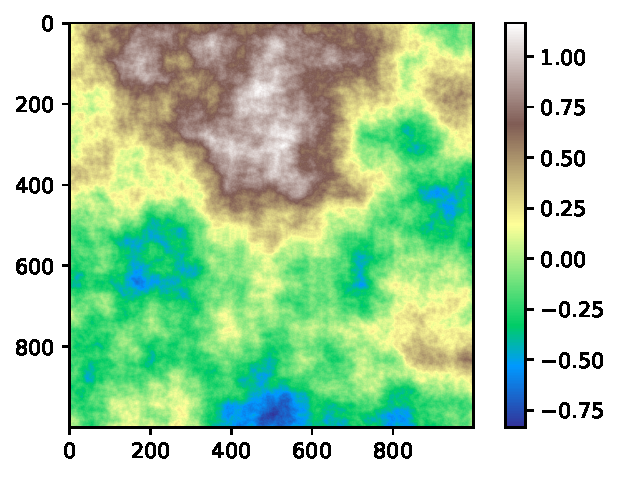
\includegraphics{MCA_files/figure-pdf/cell-2-output-1.pdf}

Para terminos prácticos del modelo

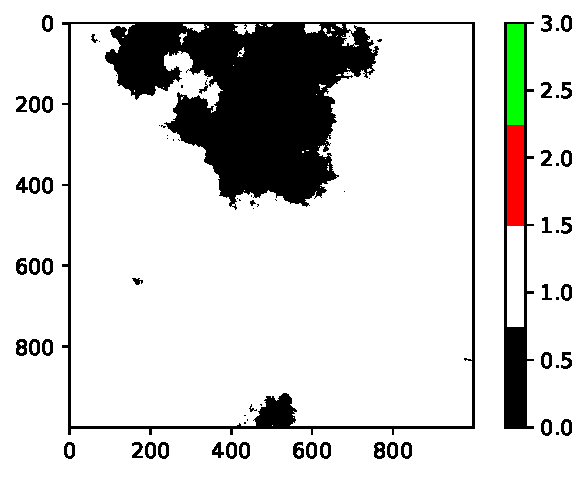
\includegraphics{MCA_files/figure-pdf/cell-3-output-1.pdf}

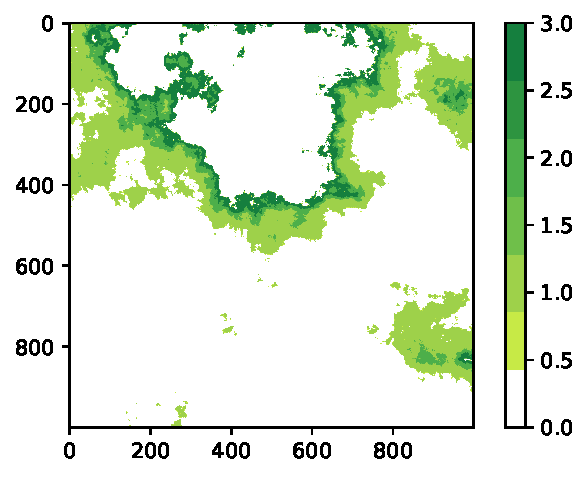
\includegraphics{MCA_files/figure-pdf/cell-4-output-1.pdf}

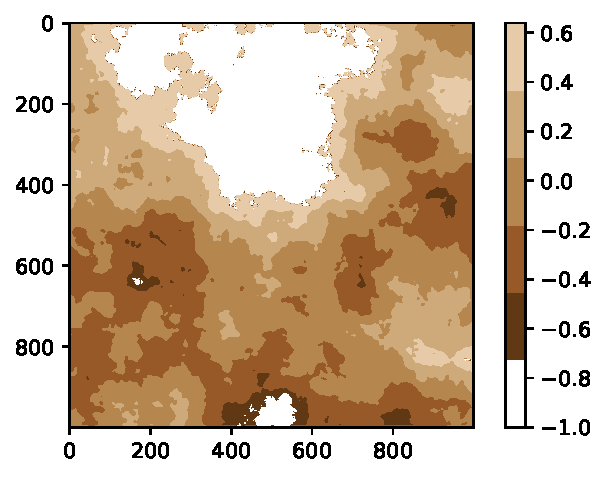
\includegraphics{MCA_files/figure-pdf/cell-5-output-1.pdf}

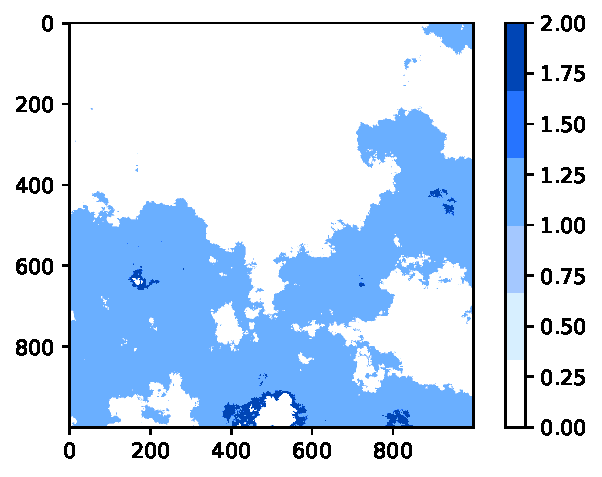
\includegraphics{MCA_files/figure-pdf/cell-6-output-1.pdf}

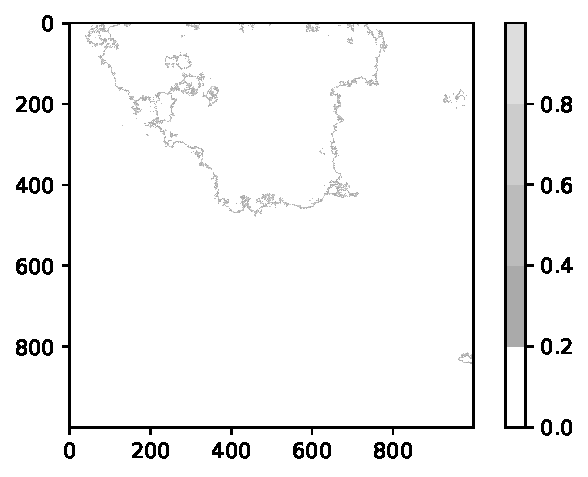
\includegraphics{MCA_files/figure-pdf/cell-7-output-1.pdf}

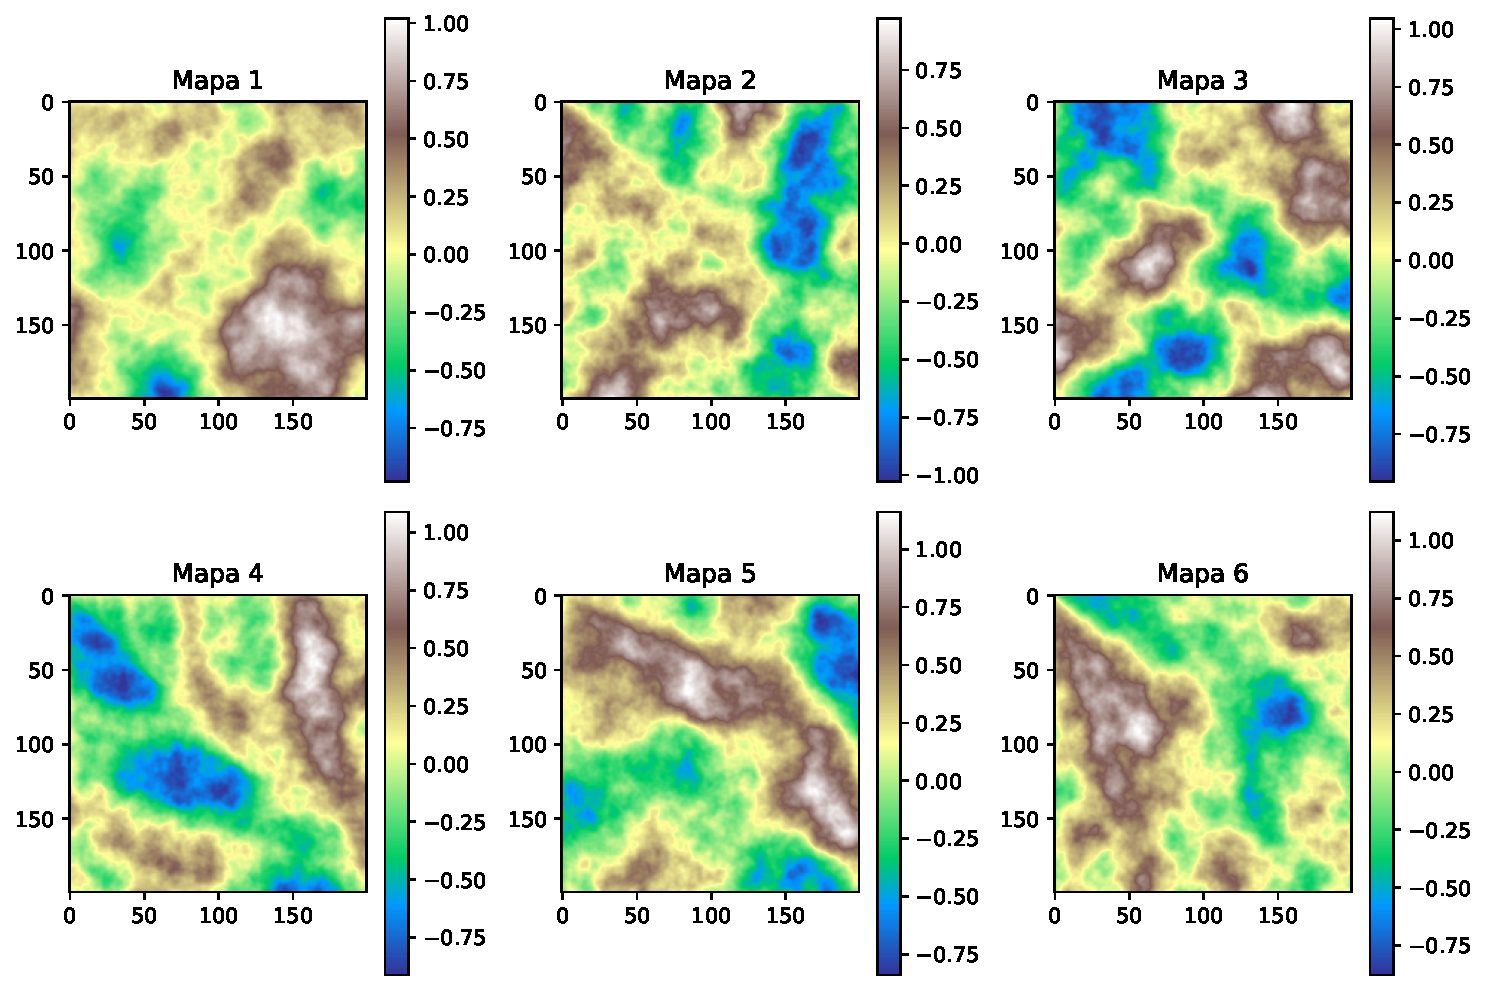
\includegraphics{MCA_files/figure-pdf/cell-8-output-1.pdf}

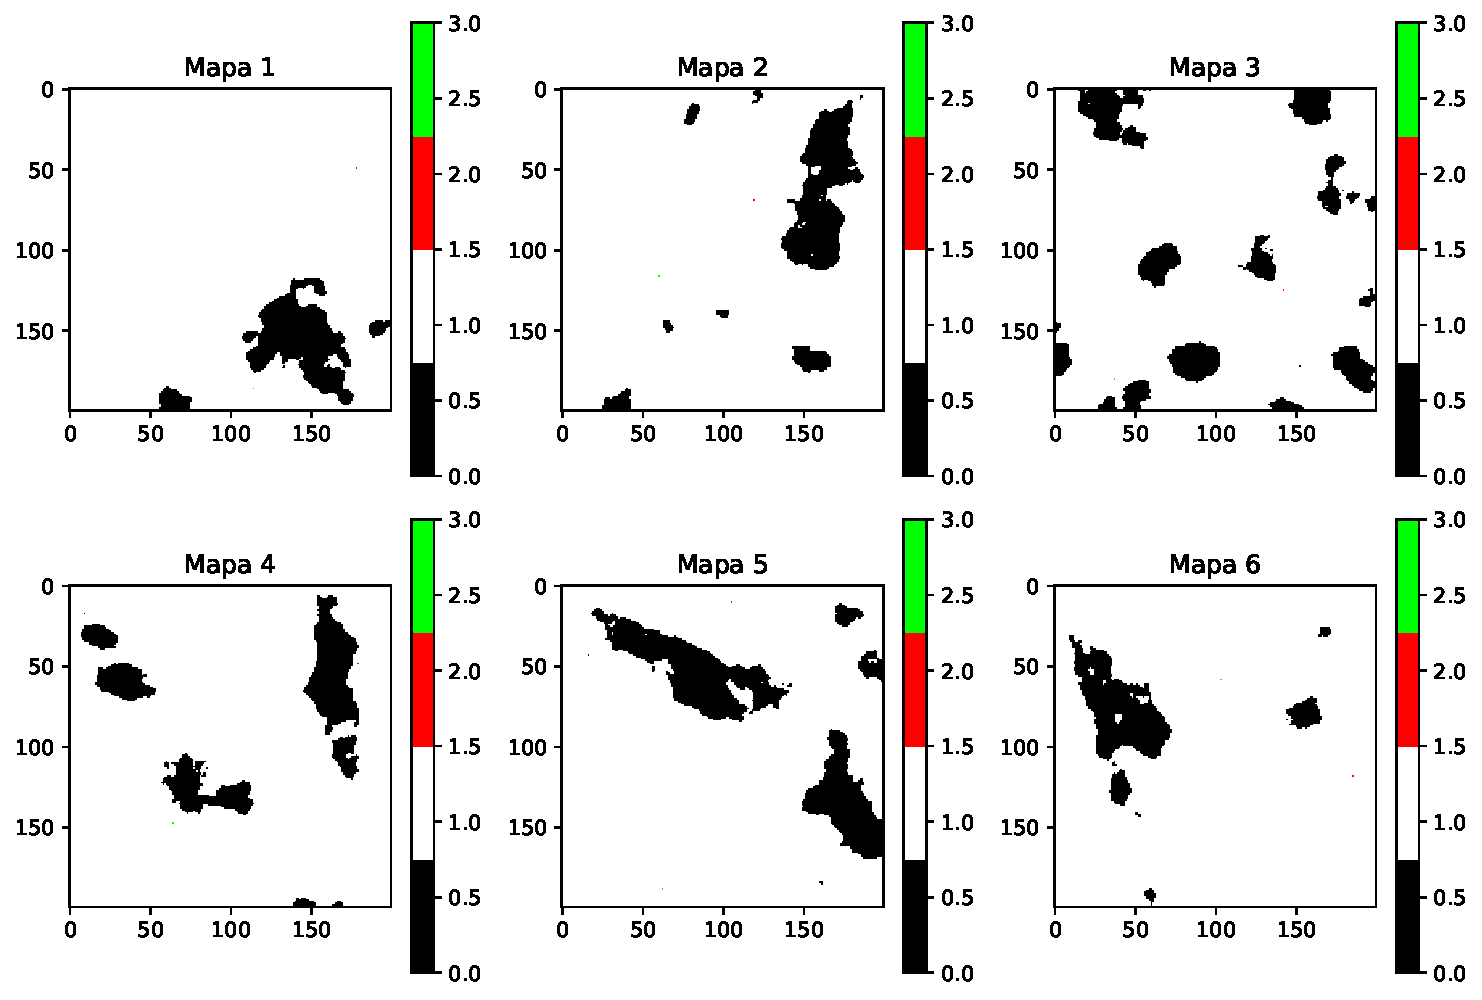
\includegraphics{MCA_files/figure-pdf/cell-8-output-2.pdf}

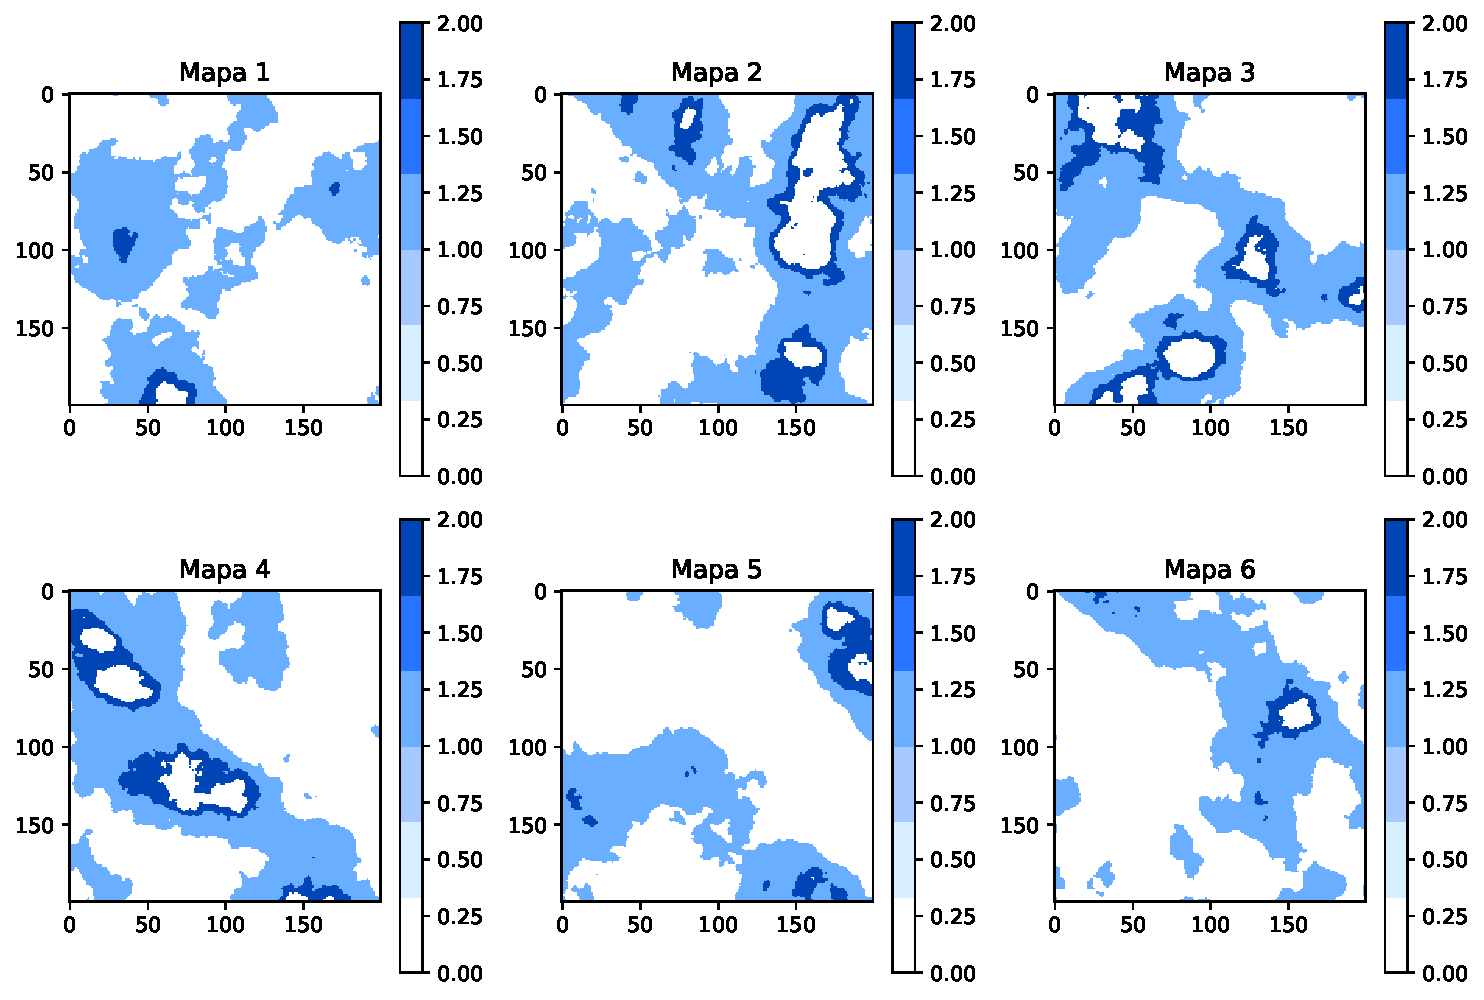
\includegraphics{MCA_files/figure-pdf/cell-8-output-3.pdf}

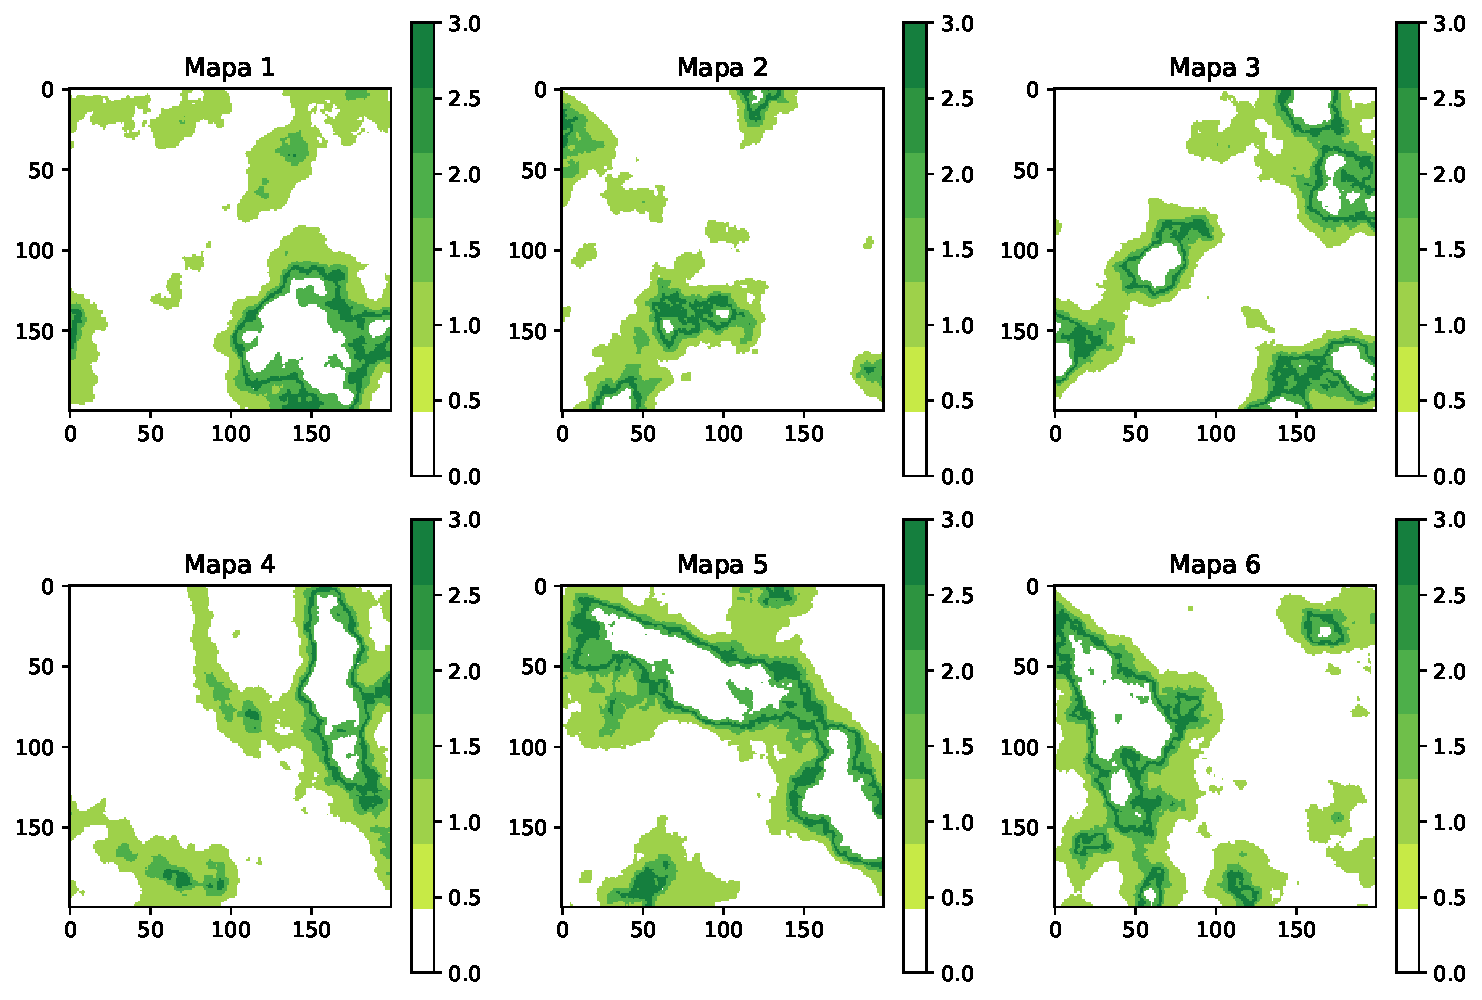
\includegraphics{MCA_files/figure-pdf/cell-8-output-4.pdf}

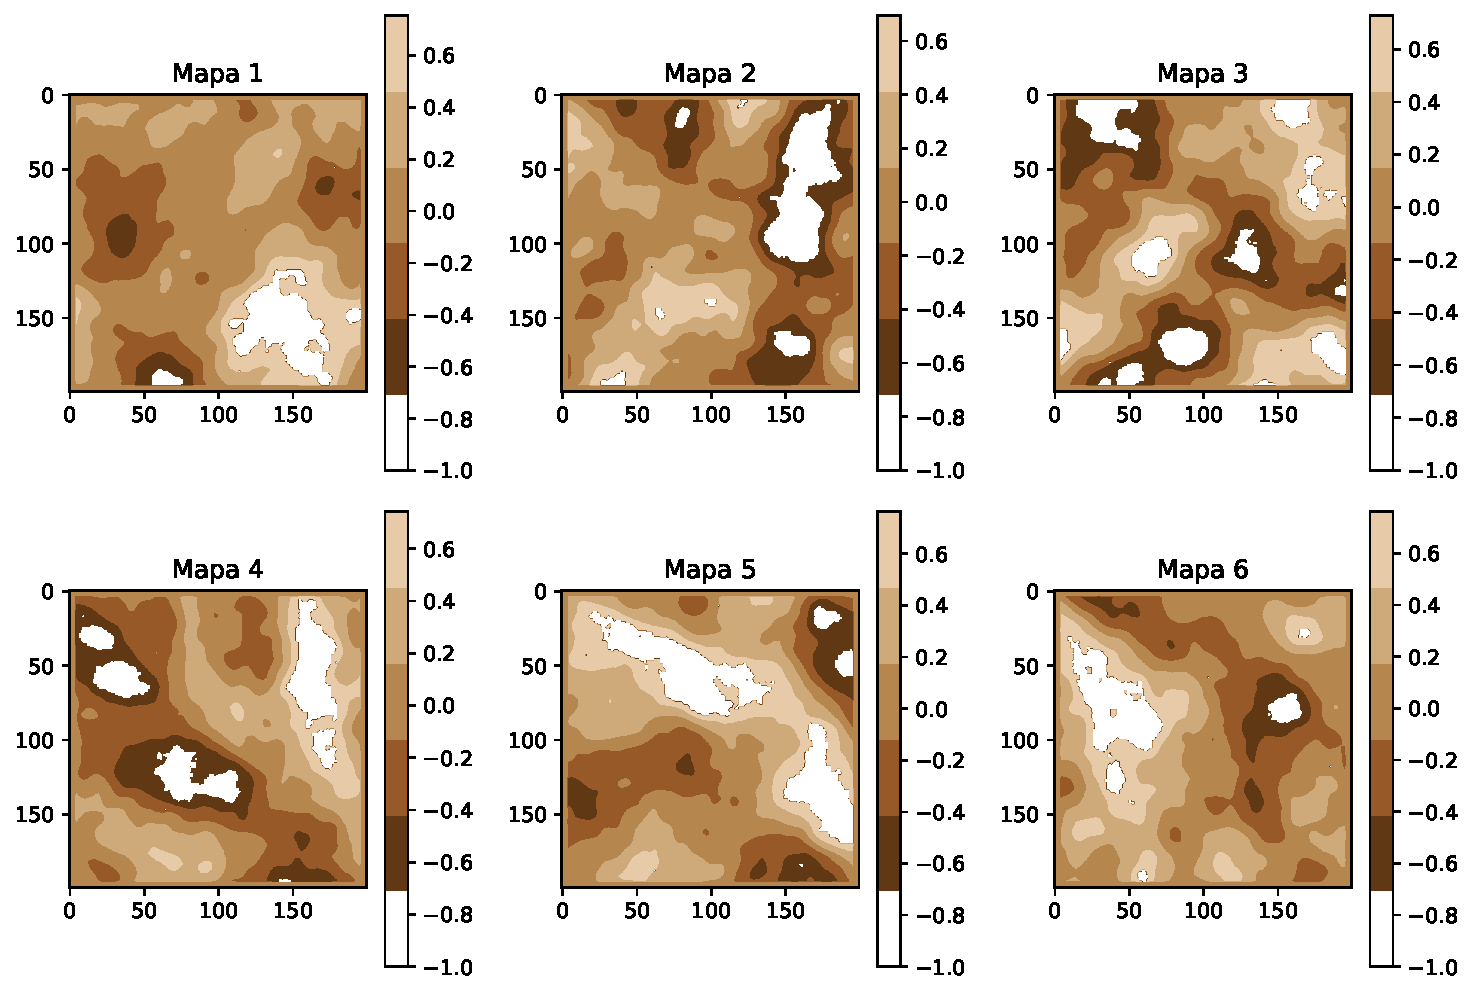
\includegraphics{MCA_files/figure-pdf/cell-8-output-5.pdf}

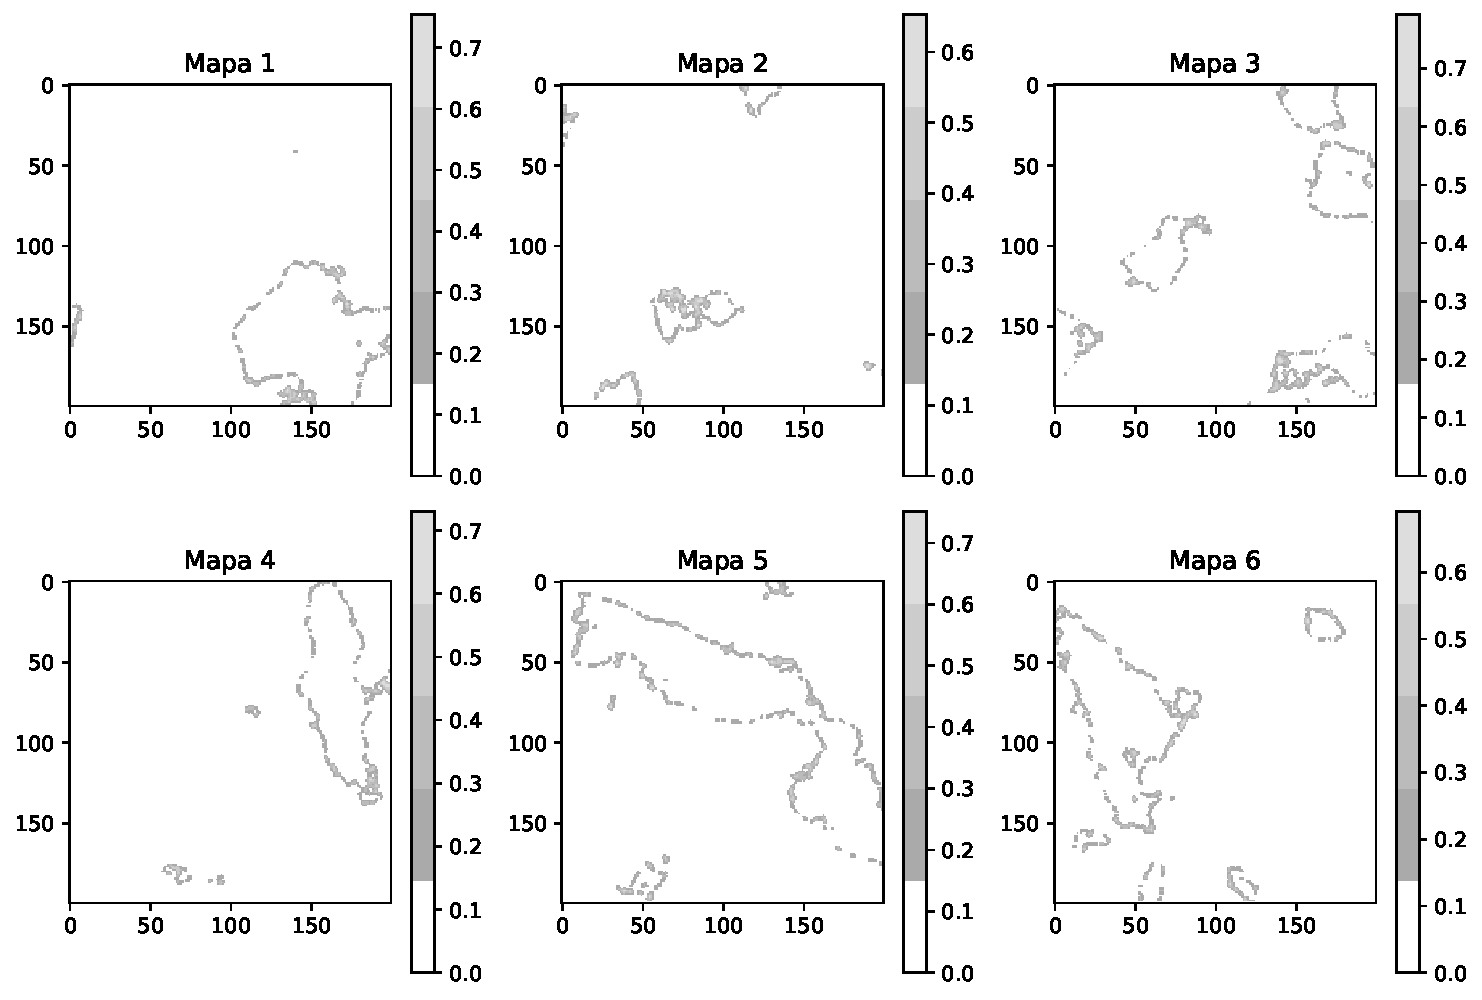
\includegraphics{MCA_files/figure-pdf/cell-8-output-6.pdf}



\end{document}
